\documentclass[12pt,letterpaper]{article}
\usepackage{fullpage, times}
\usepackage{hyperref}
\usepackage{ctable}

%% margin notes - comment out before submission
\usepackage{marginnote}
\usepackage[top=2.54cm, bottom=2.54cm, outer=5cm, inner=1.25cm, heightrounded, marginparwidth=4cm, marginparsep=0.25in]{geometry}
\renewcommand*{\marginfont}{\color{red}\small}

\bibliographystyle{jcics}

\begin{document}
\title{Deploying and Sharing QSAR Models using Predictive Modeling Markup Language}
\author{Villu Ruusmann${}^{\dagger}$ and Rajarshi Guha${}^{\ddagger}$\\
${}^{\ddagger}$National Center for Advancing Translational Sciences\\ 9800 Medical Center Drive  Rockville, MD 20850 \\ \\
${}^{\dagger}$Your address }
\date{}
\maketitle
\begin{abstract}
  A nice abstract
\end{abstract}

\section{A Plethora of Predictive Models}
\label{sec:introduction}

Quantitative Structure-Activity Relationship (QSAR) models have become
ubiquitous in computational chemistry and cheminformatics, having been
built for a variety of endpoints including biological activities and
physical properties. As shown in Figure \ref{fig:count-qsar} the last
15 years has seen a significant increase in publications developing or
using QSAR models. While there has been much discussion
\cite{Cherkasov:2014yq,Cramer2011Inevitable,Tropsha:2003aa} on the
prospective utility and validity of predictive QSAR models, a key
bottleneck to their assessment is the fact that they are not easily
obtainable. That is, the bulk of QSAR models are described in a
publication in terms of the descriptors (sometimes made available) and
the modeling method. While the implementation is noted, it is upon the
reader to actually obtain the descriptor values, obtain and set up the
modeling environment and then actually rebuild the model. In other
words, the actual model that was developed by the authors is, usually,
not available to be used directly. In a few cases, the model may be
built in a pipeline tool \cite{KNIME:2008aa}, which alleviates this
problem to some extent. Furthermore, the model development workflow
usually involves multiple software tools, each one of a specific
version. Without access to the exact same version of these tools, a
user cannot be guaranteed to exactly reproduce the model that the
authors describe. The issue of reproducibility (of workflows and
results) has become increasingly important \cite{Landrum:2012hl,
  Stodden:2013gd,Lane:2003fe} in the computational arena.

A number of workers have described infrastructure to deploy predictive
models. Some platforms such as Pipeline Pilot provide a easy to use
method to deploy a complete pipeline as a web page. However, this
approach does not allow one to share models with users who do not have
access to the software. Guha \cite{Guha:2007af} described a web based
infrastructure that allowed one to deploy serialized models developed
in R. This architecture allowed one to distribute the model via a web
page, allowing users to provide new input and retrieve
predictions. While this solution allowed the deployment of models,
they were not actually reproducible, since the serialized model did
not actually reference the input descriptors.

Bioclipse

\subsection{Model reproducibility vs. Model reusability}

When dealing with a published QSAR model, one must choose whether to
analyze its mathematical properties, or apply it to a dataset in order
to see how it performs?

One of the principles of the scientific method is that the research
must be repeatable and reproducible. From the QSAR point of view there
are not much technical obstacles in the way. The biggest concern is
using proprietary algorithms and software.

Model reproducibility is about marking down the procedure by which
the model can be derived given the same input data. Theoretical methods
do not have random error component[?]. Thus, all deviations must be
explained by systematic errors, which could be related to choosing the
wrong algorithm, wrong parametrization etc.

Documenting the whole model training and validation process with the
help of electronic laboratory notebooks. Should include both human and
machine readable instructions of the process. The latter can be given 
in the form of an executable script (ie. when executed with appropriate
input data, produces the model and output data). Plenty of options to
choose from (open source):
\begin{itemize}
  \item knitr \url{http://yihui.name/knitr/}
  \item Sweave \url{https://www.stat.uni-muenchen.de/~leisch/Sweave/}
  \item Sage \url{http://www.sagemath.org/}
  \item IPython \url{http://ipython.org/}
\end{itemize}

The ONS approach is to use Wiki pages, which contain embedded R code
and plots. For example, see
\url{http://onschallenge.wikispaces.com/MeltingPointModel002}. More
recently, websites such as
\url{https://rpubs.com/}{https://rpubs.com/} support direct web
publishing from ones local development environment.

Most of the time, however, the reader in interested in the \emph{final
ending state} of the modeling workflow. That is, the mathematical 
relationship that has been properly validated and whose applicability 
domain has been sufficiently characterized. 

\marginnote{This paragraph reads a bit too abstract. Can it be stated
  more concisely?}Essentially, the representation of a model training process boils down
to representing the training algorithm. The most complete representation
is in application code such as R, Python, MATLAB etc.
The algorithm "works" by applying a finite list of well-defined 
instructions to the initial state. After applying each instruction the
system reaches another state. When the list of instructions has been
exhausted the system has reached its final ending state.
The representation of states is technically much more challenging than 
the representation of algorithms. A state may consist of different
parts. We are only interested in that part, which relates to the 
mathematical relationship. A state can be preserved by taking a snapshot
of the particular memory area. To make reading and writing more easier,
should be formalized as a data structure.

The initial state is about the dataset. The first instructions of the
algorithm will typically split it into training and validation subsets.
A dataset can be represented using text-based database data formats such
as Comma-Separated Values (CSV), Attribute-Relation File Format (ARFF)
and others. Often becomes necessary to incorporate domain-specific
information. For QSAR, the main need is to provide the description of
the dependent field (a physicochemical property or biological activity)
and independent fields (theoretical molecular descriptors). The goal is
that if the dataset file should be "self-sustainable" if circulated
between parties. An XML-based dataset markup language called QSAR-ML [ref?].

The QsarDB approach \cite{Aruoja:2014bq,Ruusmann:2014uk} attempts to
capture the initial state, the final ending state and all states
inbetween using a collection of files in open and standard data
formats. For example, datasets are represented in TSV, parameter units
in UCUM [ref?], bibliography in BibTeX [ref?], mathematical
relationships in PMML etc. QsarDB leaves the door open for extension
information is user-defined data formats. For example, a QsarDB
archive may capture the primary model object that corresponds to the
"main" run, as well as all secondary model objects that correspond to
validation runs.

\subsection{Elements of a predictive solution}

A predictive model represents a standalone mathematical
relationship. The model itself, in terms of its mathematical form, is
not particularly easy to work with from the end user perspective. For
actual usage, a model should be packaged as a predictive solution,
which has the following components:
\begin{itemize}
  \item Data schema. Specifies information about input and output fields.
  Data schema represents the "public interface" for the end user. 
  For example, data schema could communicate that a predictive solution
  consumes a single string-type input field that contains the SMILES 
  representation of a chemical structure, and produces two output fields - 
  a string-type field that contains the classification result (eg. the 
  predicted mechanism of toxic action) and a floating point-type field 
  that contains a class-specific regression result (eg. if the chemical
  structure was classified as a narcotic agent, the predicted pIGC50 
  value using the narcosis QSAR model).
  \item Data pre- and post-processing functions. Typically, the input
  fields that are listed in data schema cannot be directly fed to the 
  underlying matchematical relationship "as is". Could be related to 
  translating input from user representation to internal representation
  (eg. converting SMILES to CDK molecular graph to CDK descriptor value)
  or performing additional transformations on it (eg. normalization, 
  converting from natural scale to logaritmic scale etc.).Similarly,
  could derive secondary output fields based on the primary field. For
  example, calculating the probability of the predicted class or standard
  error of the predicted value.
  \item Data (work)flows. A predictive solution may encapsulate more
  than one model. The passage of data from one model to another happens
  inside the predictive solution. Two most common scenarious is model 
  aggregation, where the final prediction is calculated by applying an
  aggregation function over a list of interim predictions (eg. consensus
  modeling), and model chaining, where the output of earlier models
  becomes the input of subsequent models (eg. classification followed 
  by regression).
\end{itemize}

TODO: A figure of a chemistry-specific predictive solution.

\subsection{The lifecycle of a predictive solution}

A modeling workflow has two clearly distinguishable lifecycle phases:
\begin{enumerate}
  \item Training. Happens once in the very beginning. Handled by a data
  scientist. Typically in desktop environment. 
  \item Deployment.Happens many times. Handled by plurality of IT 
  roles/personnel. Typically in server-side environment, different 
  platforms/runtimes. 
\end{enumerate}

The training is handled by a scientist. Involves analysing the
"fundamental side" of the problem, choosing the right statistical 
algorithms for training and validation. Also, providing the mechanistic
interpretation of the results (white box models). The result is 
shared with peers using modern scientific communication means. Provided
that the result is actually useful, many people may want to deploy it
on their premises afterwards.

The deployment is an operational IT problem. Different organizations 
may prefer different platforms, data frameworks. Therefore, the trained
predictive solution should be maximally portable.

The portability can be best acieved by relying on open and popular
standards. To a lesser degree, if no standards have been established yet,
could rely on open and popular tools. For example, CDK is not formally
backed by a standard, but it is generally very easy to use and integrate
with different chemistry products, because its source code can be obtained
and modified easily.

Overall, moving models from training phase to deployment phase is a
major hurdle in practical data science. It is estimated that in corporate
environments the average length of a modeling iteration may be as long
as 16-24 months [private conversation, public ref?]. All approaches that
can reduce this timespan and associated costs could provide significant
business value.

\subsection{Representation of models}

It is possible to distinguish between three levels:
\begin{itemize}
  \item Data structure. Tied to a specific library and/or algorithm.
  For example, the \textit{randomForest} R library returns the trained
  RF model as a special-purpose data structure. Moreover, the internal
  structure of this data structure varies depending on whether the RF
  model was trained using the "formula interface" or the "matrix interface".
  Such data structures can be easily persisted into files using so-called
  serialization mechanisms. The storing operation (ie. saving the in-memory
  data structure to disk file) is called serialization, and the loading
  operation (ie. reading the disk file data structure to memory) is called
  deserialization. Most language runtimes provide built-in serialization
  capabilities. For example, R language provides methods \textit{saveRDS}
  and \textit{readRDS} that can work with binary and text-based files.
  \item Pseudocode. A similar model can be trained using different libraries
  and/or algorithms. For example, a RF model can also be trained using
  the \textit{party} R library (or in-house R library). The choice of the
  algorithm determines how the search is conducted in the feature space. 
  However, the final ending state of a RF training process is an ensemble
  of decision tree models.
  The goal of the pseudocode representation is to extract and encapsulate
  the primary structure of the model. The pseudocode representation aims 
  to be much more informative for humans (eg. following the computation
  path from beginning to end), but still be directly interpretable by 
  machines. For example, a decision tree model could be represented by
  a tree-like data structure, where non-leaf nodes specify split criteria 
  and leaf nodes specify predicted scores.
  \item Application code.\marginnote{Its not clear what this level
      means. Are you making a distinction between 'interpretation' and
      'compilation'? It seems data structures or pseudocode both end
      up as application code at one point}During deployment, the model is executed with
  with new input data. With data structure and pseudocode approaches this 
  is accomplished by model interpretation. The alternative approach is to
  translate either representation to application code, which would allow
  for more optimizations and much speedier execution. 
\end{itemize}

Binary serialization mechanisms are usually more performant and 
compact compared to text based methods. The primary disadvantage is
that they cannot be manually inspected and require special tools to
parse and view them.

The choice of serialization data format depends whether model producer 
and model consumer will be using the same language platform or not. For
example, the RDS data format that is default for R language is not very
suitable when model consumer is a Java or Python application. Today,
there are plenty multi-platform serialization data formats that offer
bindings for most popular programming languages:
\begin{itemize}
  \item Protocol Buffers \url{https://code.google.com/p/protobuf/}
  \item Apache Avro \url{http://avro.apache.org/}
  \item XML
  \item JSON
  \item YAML
\end{itemize}

The first step towards pseudocode would be to have shared data structures.
For example, from the model deployment perspective it would be desirable
if the \textit{randomForest} and \textit{party} libraries were using common
data structure for the representation of decision trees. In practice,
however, it is pretty difficult to accomplish it without a third-party 
standardizing body. The responsibilities of such third party would be 
then to specify, develop and maintain an independent library that could
be imported on demand. The key issue is obtaining acceptance and support
by major tool vendors in the field. Moreover, this library of "common 
data structures" does not have to be limited to one specific language, but
be applicable across all platforms and languages that are used for
everyday statistics and machine learning work.

The predictive analytics community has decided to standardize around
the Predictive Model Markup Language (PMML) [ref?], which is an XML-based
markup language for the representation of predictive solutions. 

\subsection{Serializing Models}
\label{sec:serializing-models}

A key step in sharing predictive models is serialization. That is,
converting the internal representation of the model developed in some
environment (R, Weka, Matlab, Mathematica etc) to a disk file (usually
a sequence of bytes). Not all deployment approaches require this step
- usually platforms that host the deployment and development
mechanisms (e.g., Pipeline Pilot, R using Shiny [REF]). But in general, for one to share a
model, it must be serialized and the serialized form is exchanged.

Most model development platforms support binary serialization
schemes. For example, R can save models in the RData format [REF]
which is binary and can only be read by the R platform (though since
it is Open Source, one could read/write such files using custom
code). XXX What about Matlab? XXX Java objects (say from Weka) can
be serialized using the Java Object Protocol [REF http://docs.oracle.com/javase/7/docs/technotes/guides/serialization/]

In contrast to binary serialization formats, the Predictive Modeling
Markup Language is a plain text XML format that is designed to fully
describe the model. Importantly, with appropriate software a PMML
document can be used to reconstruct the model, including any data
preprocessing steps (scaling, normalization) as well as generate input
descriptors if appropriately specified. A number of software tools are
capable of reading and writing PMML documents including SAS, SPSS,
TIBCO and KNIME, whereas others such as R can produce PMML documents
and WEKA which can consume PMML documents.

\ctable[cap={}, caption={Growth in number of Pubmed articles that use the term QSAR.},
label={fig:count-qsar},figure,botcap]
{c}
{}
{
  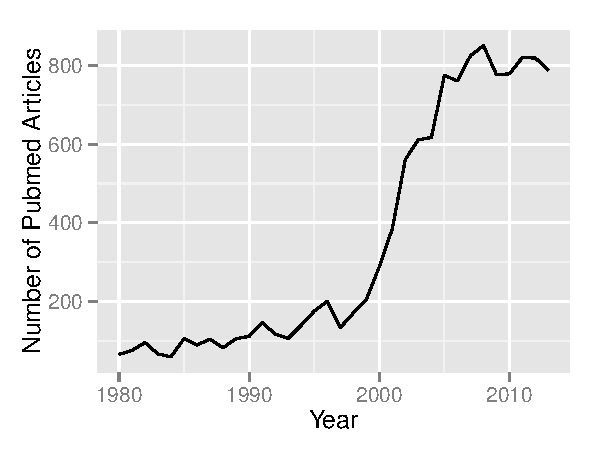
\includegraphics{img/count-qsar}
}

\subsection{Representation of descriptors}

A molecular descriptor is a characteristic that is obtained by applying
a particular algorithm to a particular chemical structure representation.
Typically classified by the complexity of the structure representation:
\begin{enumerate}
  \item 1D - Atom and bond counts and other constitutional features
  \item 2D - Atom-atom connectivity
  \item 3D - Conformation dependent, 3D atom coordinates
\end{enumerate}

Descriptor calculations can be difficult to reproduce. This is
primarily driven by differences in the chemistry models implemented in
different toolkits and chemical software platforms. An example is the
count of aromatic carbons - which is dependent on the aromaticity
model (of which there are several) employed by the implementation. As
a result, while descriptors calculated using a given toolkit are
reproducible, this is only guaranteed within that \emph{specific
  version} of the toolkit. The same algorithm may give different
results using another cheminformatics toolkit.

\marginnote{This paragraph seems to digress a little and doesn't
  really focus on the issue at hand}By definition, when the algorithm
is applied to an incorrect chemical structure representation, the
results is an incorrect molecular descriptor value. Cannot reliably
say if an user-specified representation is correct or not by merely
"looking" at it. Will need to apply a rigorous verification
procedure. For example, suppose SMILES chemical structure
representation.  There exist different variations of SMILES, some of
which make aromaticy transparent by using different atom and bond
symbols (ie. lowercase letter "c" and/or carbons connected by ":"
bonds). Therefore, simple analysis of SMILES using simple text
analysis functions won't suffice, and it has to be parsed and
reconstructed into more sophisticated chemical graph. Even then it is
possible to run into trouble, because the ring detection and ring
aromaticity assignment can be performed following different
algorithms.

\marginnote{Is it really the case that the structure representation is
  the issue? Shouldn't any decent standardization tool transform multiple
  input forms to a single canonical form?}Due to these issues,
providing a ``complete'' QSAR models to an end-user requires that we
specify the supported input chemical structure representations. Most
likely, actual chemical databases contain chemical compounds in data
formats that cannot be fed \emph{directly} to the molecular descriptor
calculation algorithm. For example, when testing with new chemical
compounds then user input may originate from graphical drawing board
(eg. JMol applet [ref?] or J(S)ME Java(Script) Molecular Editor applet
[ref?]) or be a systematic name. The desirable property of a QSAR
predictive solution would be to recognize and automatically convert
between different chemical structure representations.

Unlike model training algorithm, the molecular descriptor calculation
algorithm does not have intermediary reusable states. From the practical
point of view, can be only reused by providing the complete algorithm in 
the application code form.

There have been attempts to "simplify" the systematizing and
communicating algorithms using the ontology approach. The earliest
work is the Blue Obelisk Descriptor Ontology \cite{Guha:2006ac}, which
has been now superseded by the Chemical Information (CHEMINF) Ontology
\cite{Hastings:2011rf}.

\marginnote{Probably not useful to speak negatively (at least in this
  article). Maybe drop this paragraph or just simplify
  it}Unfortunately, not much adoption, because the vocabulary of
real-life algorithms is way beyond the standardized vocabularies, and
the lack of competing implementations. An ontology that has been
crafted following CDK data structures and concepts is unlikely to be
relevant and useful for other descriptor calculation software. In
other words, if there is an one-to-one correspondence between ontology
identifiers and CDK implementation classes, then it may be a better
idea to give those CDK class names directly, and avoid the
intermediary layers of "ontology identifiers" altogether.

The challenges of formalizing algorithm descriptions using ontologies
is well demonstrated by the ``parametrization problem''.  That is, the
behaviour of most algorithms can be tweaked by adjusting a set of
control variables or parameters. For example, one approach to 3D
analysis of molecular shape requires one to specify a mesh
size. Different values represent trade-offs between speed and accuracy
and will lead to different descriptor values. Thus a full
specification of an algorithm must also include the details of the
parametrization. Encoding this level of detail in an ontology may not
be appropriate.

\marginnote{This is always a possibility - not sure whether its worth
  mentioning}Another source of "variance" for molecular descriptor
algorithms are programming errors. It is possible that newer versions
of the same software could yield different results than older
versions, because the algorithm has been slightly changed (or
reparameterized) in some point in time.

\section{Methods}
\label{sec:methods}

\subsection{Model Development}
\label{sec:model-development}

For this study we developed models in R 3.1 [REF] with descriptors
generated using the CDK \cite{Steinbeck:2003bh} via the rcdk
\cite{Guha:2007aa} package. As exemplars we considered two
datasets. XXX Describe the datasets.

Next we developed a linear regression (or classification) and random
forest  model  for each dataset. Using the pmml package [REF] we
serialized the models to PMML.

\subsection{Model Deployment}
\label{sec:model-deployment}


\section{Discussion}
\label{sec:discussion}

\subsection{PMML Supports Open Science}
\label{sec:pmml-supports-open}



\bibliography{paper}

\end{document}
